% ----------------------------------------------------------
% \documentclass[svn, draft]{rureport}
\documentclass[svn, final]{rureport}
% ----------------------------------------------------------
\svnid{$Id: example-techreport.tex 48 2014-10-23 15:40:52Z foley $}
% if you'd like the above information to be updated,
% use svn properties to set svn:keywords to for Id and URL (or HeadURL)
% Don't forget to set the draft to final before submitting

%% The default fixmes are:  \fxnote{} \fxwarning{} \fxerror{} \fxfatal{} (same as \fixme{})
% if you want personalized fixmes, then register the authors here
% notice that the first field is 2 letters, the second is 3.
\FXRegisterAuthor{jf}{jtf}{foley}
% this registers \jfnote{}, \jfwarning{}, \jferror{}, \jffatal{}

%% declare the paths(s) where you graphics files can be found
\graphicspath{{graphics/}{Graphics/}{./}}

\author{Ásbjörn~Kristinsson,~Andrés~Laverde,~Yaroslav~Pyshakov}  % My name, for the titlepage
\title{Electricity monopolies in Iceland}  % The title, for the titlepage
\course{Energy Economics and Policy - Dominic Scott}

\usepackage{float}
\floatstyle{plaintop}
\restylefloat{table} % Place table caption above

\usepackage{url}
\usepackage{amsmath}
\usepackage{wrapfig}
\usepackage{parskip}
\setlength{\parindent}{0pt}
\usepackage{gensymb}
\usepackage{caption}
\usepackage{bm}
\usepackage{multicol}
\usepackage{hyperref} % must be last package loaded!
% it makes hyper-references (citations, URLs, etc) clickable

\begin{document} % this tells the compiler that it is time to make
                 % text to print instead of just getting ready.
\maketitle  % make a title page from the Title, Date, and Author
\listoffixmes{}
%\section*{Errata} %%section* avoids putting a number 
%--------------------------------------------------------------%
%------------------------ INTRODUCTION ------------------------%
%--------------------------------------------------------------%

\section{Introduction to the Icelandic energy market}

Monopolies occur when a company and its product offerings dominate a sector or industry. They can be considered an extreme result of free-market capitalism with an absence of restrictions or restraints. Consequently, a single company or group becomes large enough to own all or nearly all the market for a particular type of product or service. The term monopoly is often used to describe an entity that has total or near-total control of a market. There are three types of them: natural, state monopoly and un-natural monopoly. 

The Icelandic electricity grid is governed by a relatively liberalised regulatory framework. However, the generation and transmission parts show characteristic features of monopolies. Almost 100\% of electricity is generated using hydropower and geothermal energy; therefore, most hydropower plants are owned by one dominant state-owned company, Landsvirkjun. On the other hand, the transmission system is ruled by the Icelandic law to be operated by only one company, Landsnet, which is also a state-owned firm and oversees the operation, maintenance and economic aspects of electricity transmission. The distribution network is quite liberalised and has various market players in it. This situation configures a competitive retail market where customers are free to choose their provider. The Icelandic electricity grid is mapped out in figure ---, exhibiting the companies that are part of the network in each sector of the market. 



\begin{figure}[h!]
    \centering
    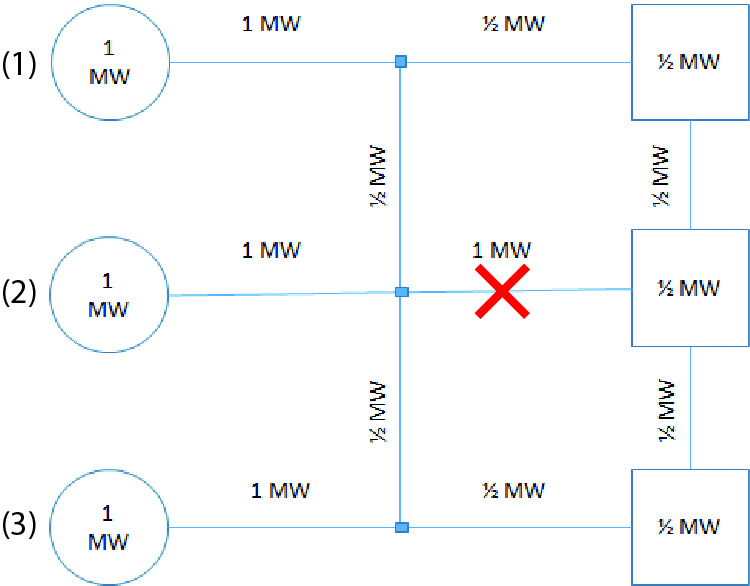
\includegraphics[width=0.6\linewidth]{N-1.jpg}
    \caption{Power network diagram showing the loss of the 1MW line in the middle of the grid.}
    \label{fig:N-1}
\end{figure}

The regulatory framework is established in the Electricity Act No. 65 of 2003 [2] where the Alþingi sets the parameters for an economical, reliable, secure and efficient electricity system. The Electricity Act also lists the rights and duties that companies have, being effective in the generation, transmission, distribution and trade systems. This legislation is fully covered by EU directives, especially the Directive 72/EC of the European Parliament and of the Council of July 13th of 2009 [5]. The Directive’s objective is to achieve an unbundled energy market where competition ensures the security of supply and the most competitive prices. 

This paper aims to provide an insight into the monopolies present in the Icelandic electricity market, assessing the features of each sector of the electricity network. For this, it is necessary describe the type of monopoly in each part of the grid, as well as evaluate the competitiveness in the market. 

\subsection{Generation}

According to the Electricity Act, the generation side is ruled as a competitive market where companies apply for a license to operate [2]. Here, Landsvirkjun is a player in a competitive market [1] in which generation is carried out by various competitors. However, Landsvirkjun owns around 70\% of the electricity generation, making it less clear about the nature of this part of the market. Since one firm is responsible for the production of more than two-thirds of the output, it should be noted that this could lead to the constitution of a natural monopoly. The competitive nature of the generation market leaves the roles of Landsvirkjun unclear and therefore leads to a relatively unfair competition [1].

\subsection{Transmission}

The Electricity Act has ruled that “only one company shall be responsible for the transmission of electricity and system management” [2]. This operation is carried out by Landsnet, configuring a natural monopoly. The reason behind the establishment of only one transmission company lies in the concept of economies of scale. Transmission of electricity requires high capital costs for initial investment and maintenance of the system. This enforces licensing only one company to operate such a system, in a way that it results economically for it, for the generators and consumers and for the country itself. Thus, the law promotes a natural monopoly in order to enhance the allocation of welfare and efficiency of the electricity network. For this, the Electricity Act imposes strong regulations on Landsnet to prevent it from setting high prices to distributors and end consumers, and to ensure a good operation of the transmission system. 

\subsection{Distribution}

\subsection{Retail and wholesale markets}

The retail and wholesale markets are relatively competitive networks where Landsvirkjun also participates. Six companies supply energy to end consumers and they are provided by the wholesale market dominated by Landsvirkjun, as shown in the graph ---. Landsvirkjun covers 55\% of this part of the market and the remaining portion is shared by Orka náttúrunnar, HS Orka, Orkusalan and others. The amount of electricity that Landsvirkjun provides to the distribution companies is comprised within the wholesale market [6].

%--------------------------------------------------------------%
%-------------------------- PRICING ---------------------------%
%--------------------------------------------------------------%

\section{Electricity pricing}

%--------------------------------------------------------------%
%------------------------- REGULATION -------------------------%
%--------------------------------------------------------------%

\section{Regulation, competitiveness and market and operative efficiency}

According to the Electricity Act of Iceland, and more generally to the Directive 72 of 2009 of the European Union, the main objective is to reach an energy market where a competitive environment promotes innovation, fair pricing and efficient operation. One of the goals of the regulations for the effective unbundling of the market is to remove the incentives for vertically integrated companies. A consequence of this is the disintegration of monopolies in the energy sector [5]. Iceland has embraced the standards of liberalisation permitting the entrance of competitors to the generation system, as well as to the distribution system. Nonetheless, the generation part of the market exhibits limited competition due to the presence of a dominant player. The transmission system, on the other hand, is a natural monopoly where only Landsnet is authorized to operate it.

\subsection{Assessment of the generation market}

On the generation side, Landsvirkjun is responsible for the generation of approximately 70\% of the electricity, making it the largest competitor. Due to the nature of the electricity market, Landsvirkjun faces low competitive pressure from other enterprises and this could lead to market and operational inefficiencies [1]. Although they are not currently present, it is worth noting that the lack of strong competitors could produce lower innovation efforts from the dominant company [3].  Additionally, the dominant position of Landsvirkjun generates a risk of unfairness in the market because the company could set the prices too high (e.g., higher than the marginal cost of production) compared to the optimal welfare [6]. This also configures a risk situation where there could be indirect subsidies from the transmission system operator to Landsvirkjun or transfer pricing [6].   
The regulatory framework contained within the Electricity Act and monitored by Orkustofnun prevents the “abuse of dominance” of the biggest generator by enforcing it to make public the wholesale prices of electricity [7]. This regulation drives the company to improve pricing towards equity, enhancing, therefore, market efficiency, transparency and allocation of welfare. Moreover, making electricity contracts with power-intensive customers is a way of entering global competition [6]. The negotiation of new projects for providing electricity to new intensive consumers increases the competitive nature of the market on a regional scale. Consequently, this action reduces the risk of precarious decisions made by Landsvirkjun and a malfunctioning market. 

\subsection{Assessment of the transmission market}

Among the regulations for electricity transmission, a revenue cap is imposed on Landsnet set by Orkustofnun to prevent it from setting marginal cost pricing. Based on this revenue cap, Landsnet prepares its transmission tariffs applied to general and power-intensive users, reflecting the value of the product that is being delivered. The tariffs are simply based on the electricity that distributors or power-intensive users draw from the grid. They are divided into three different charges: the delivery charge, which includes individual connections to the transmission system; the capacity charge, which is calculated based on the average of the four highest 60-minute monthly power-peaks of the year; and the energy charge, calculated for each MWh transferred through the transmission grid [4]. Consequently, these tariffs reflect the real-time market prices, they are transparent accordingly to the costs and value of the product and contribute to high market efficiency. 

Even though the transmission exhibits an obvious lack of competition, regulatory policies are effective when it comes to the balance between electricity pricing and return in relation to capital costs. The reason for maintaining only one company in the operation of the transmission is to ensure market efficiency, given that electricity requires massive economies of scale. Thus, a monopoly like Landsnet guarantees fair trading of electricity for both general and power-intensive consumers with good allocative efficiency. Furthermore, a similar situation to Landsvirkjun occurs with Landsnet when it comes to entering the global market by trading energy contracts with power-intensive consumers. A fairer market evolves from the competition inside regional markets by attracting intensive users. 

\subsection{Assessment of the distribution market}

The distribution system is legislated in a way that the government provides licenses to different companies to operate in different distribution zones. Therefore, distribution is a competitive system where diverse companies are in charge of providing electricity to retail consumers. The distribution system operators set their tariffs in each distribution zones with prior approval of Orkustofnun, including the costs of transmission and distribution [2, 9]. The final consumers adopt these rates, and they are free to choose their supplier. Even though the distribution system is considered a competitive market on a national level, it is thought microeconomically as zoned natural monopolies [6, 9, 10]. As distributors operate as a unique company in certain regions, the regulator should benchmark them relative to the other companies to supervise good functioning of the system and improve the efficiency of the distributors [6]. 

Competitiveness in the retail market is limited due to restricted price transparency. Some the retailers are vertically integrated, and they derive they retail electricity from the generation arm of the principal firm or buy electricity from the other retailers. This creates an environment of low transparency because there is no trade between the different generator companies and retailers [8]. Moreover, the generation of electricity by companies apart from Landsvirkjun is not sufficient to cope with the load, making it necessary to resort to Landsvirkjun’s wholesale. The dependency of the other companies of Landsvirkjun and the vertical affairs make the competition in the retail market limited and non-transparent. 

% ------------------------------------------------------
% --------------------  REFERENCES  --------------------
% ------------------------------------------------------
\newpage
% \section{References}

%If you are testing Biber/Biblatex, this citation contains Icelandic characters \cite{foley2013dustcloud}

\bibliographystyle{IEEEtran}
\bibliography{references}

% ------------------------------------------------------
% ---------------------  APPENDIX  ---------------------
% ------------------------------------------------------
% Uncoment this for appendix
%\newpage
%\appendix
%\section{Design documents}
%Put CAD drawings, additional sketches

\end{document}
%%%%%%%%%%%%%%%%%%%% TeXStudio Magic Comments %%%%%%%%%%%%%%%%%%%%%
%% These comments that start with "!TeX" modify the way TeXStudio works
%% For details see http://texstudio.sourceforge.net/manual/current/usermanual_en.html   Section 4.10
%%
%% What encoding is the file in?
% !TeX encoding = UTF-8
%% What language should it be spellchecked?
% !TeX spellcheck = en_US
%% What program should I compile this document with?
% !TeX program = latex
%% Which program should be used for generating the bibliography?
% !TeX TXS-program:bibliography = txs:///bibtex
%% This also sets the bibliography program for TeXShop and TeXWorks
% !BIB program = bibtex

%%% Local Variables:
%%% mode: latex
%%% TeX-master: t
%%% End:
